\documentclass[10pt]{article}
\usepackage[margin=1cm]{geometry}
\geometry{a4paper}

\usepackage{fontawesome}
\usepackage[dvipsnames]{xcolor}

\usepackage{tikz}
\usetikzlibrary{patterns}
\usetikzlibrary{patterns.meta}

\pagestyle{empty}

\begin{document}

\begin{center}
\begin{tikzpicture}
  % PLAYER A
  \node[] at (-5,-1.25) {\parbox{5cm}{\centering \sffamily \Large \color{BrickRed} \textbf{Player A}}};
  % PLAYER A, NUMBER 1
  \node[] at (-5,-2.75) {\parbox{5cm}{\sffamily \large \color{BrickRed}
  %%%[LEVEL DESCRIPTION HERE: PLAYER A, NUMBER 1]%%%
  }};
  \node[] at (-5,-6) {%
  %%%[PUZZLE HERE: PLAYER A, NUMBER 1]%%%
  };
  % PLAYER A, NUMBER 2
  \node[] at (-5,-10.75) {\parbox{5cm}{\sffamily \large \color{BrickRed}
  %%%[LEVEL DESCRIPTION HERE: PLAYER A, NUMBER 2]%%%
  }};
  \node[] at (-5,-14) {%
  %%%[PUZZLE HERE: PLAYER A, NUMBER 2]%%%
  };
  % PLAYER A, NUMBER 3
  \node[] at (-5,-18.75) {\parbox{5cm}{\sffamily \large \color{BrickRed}
  %%%[LEVEL DESCRIPTION HERE: PLAYER A, NUMBER 3]%%%
  }};
  \node[] at (-5,-22) {%
  %%%[PUZZLE HERE: PLAYER A, NUMBER 3]%%%
  };
  %
  \node[] at (-5,-26.5) {\parbox{5cm}{\centering \sffamily Puzzle~\#%
  %%%[PUZZLE SET ID HERE: PLAYER A]%%%
  }};
  % PLAYER B
  \node[] at (5,-1.25) {\parbox{5cm}{\centering \sffamily \Large \color{BrickRed} \textbf{Player B}}};
  % PLAYER B, NUMBER 1
  \node[] at (5,-2.75) {\parbox{5cm}{\sffamily \large \color{BrickRed}
  %%%[LEVEL DESCRIPTION HERE: PLAYER B, NUMBER 1]%%%
  }};
  \node[] at (5,-6) {%
  %%%[PUZZLE HERE: PLAYER B, NUMBER 1]%%%
  };
  % PLAYER B, NUMBER 2
  \node[] at (5,-10.75) {\parbox{5cm}{\sffamily \large \color{BrickRed}
  %%%[LEVEL DESCRIPTION HERE: PLAYER B, NUMBER 2]%%%
  }};
  \node[] at (5,-14) {%
  %%%[PUZZLE HERE: PLAYER B, NUMBER 2]%%%
  };
  % PLAYER B, NUMBER 3
  \node[] at (5,-18.75) %{\parbox{5cm}{\sffamily \large \color{BrickRed} }};
  {\parbox{5cm}{\sffamily \large \color{BrickRed}
  %%%[LEVEL DESCRIPTION HERE: PLAYER B, NUMBER 3]%%%
  }};
  \node[] at (5,-22) {%
  %%%[PUZZLE HERE: PLAYER B, NUMBER 3]%%%
  };
  %
  \node[] at (5,-26.5) {\parbox{5cm}{\centering \sffamily Puzzle~\#%
  %%%[PUZZLE SET ID HERE: PLAYER B]%%%
  }};
  %
  \draw[] (0,0.5) edge[ultra thick, dashed] (0,-27);
  \node[fill=white,inner sep=0pt] at (0,-26.2) {\rotatebox{90}{\Huge \faScissors}};
  %
\end{tikzpicture}
\end{center}

\pagebreak

\begin{center}
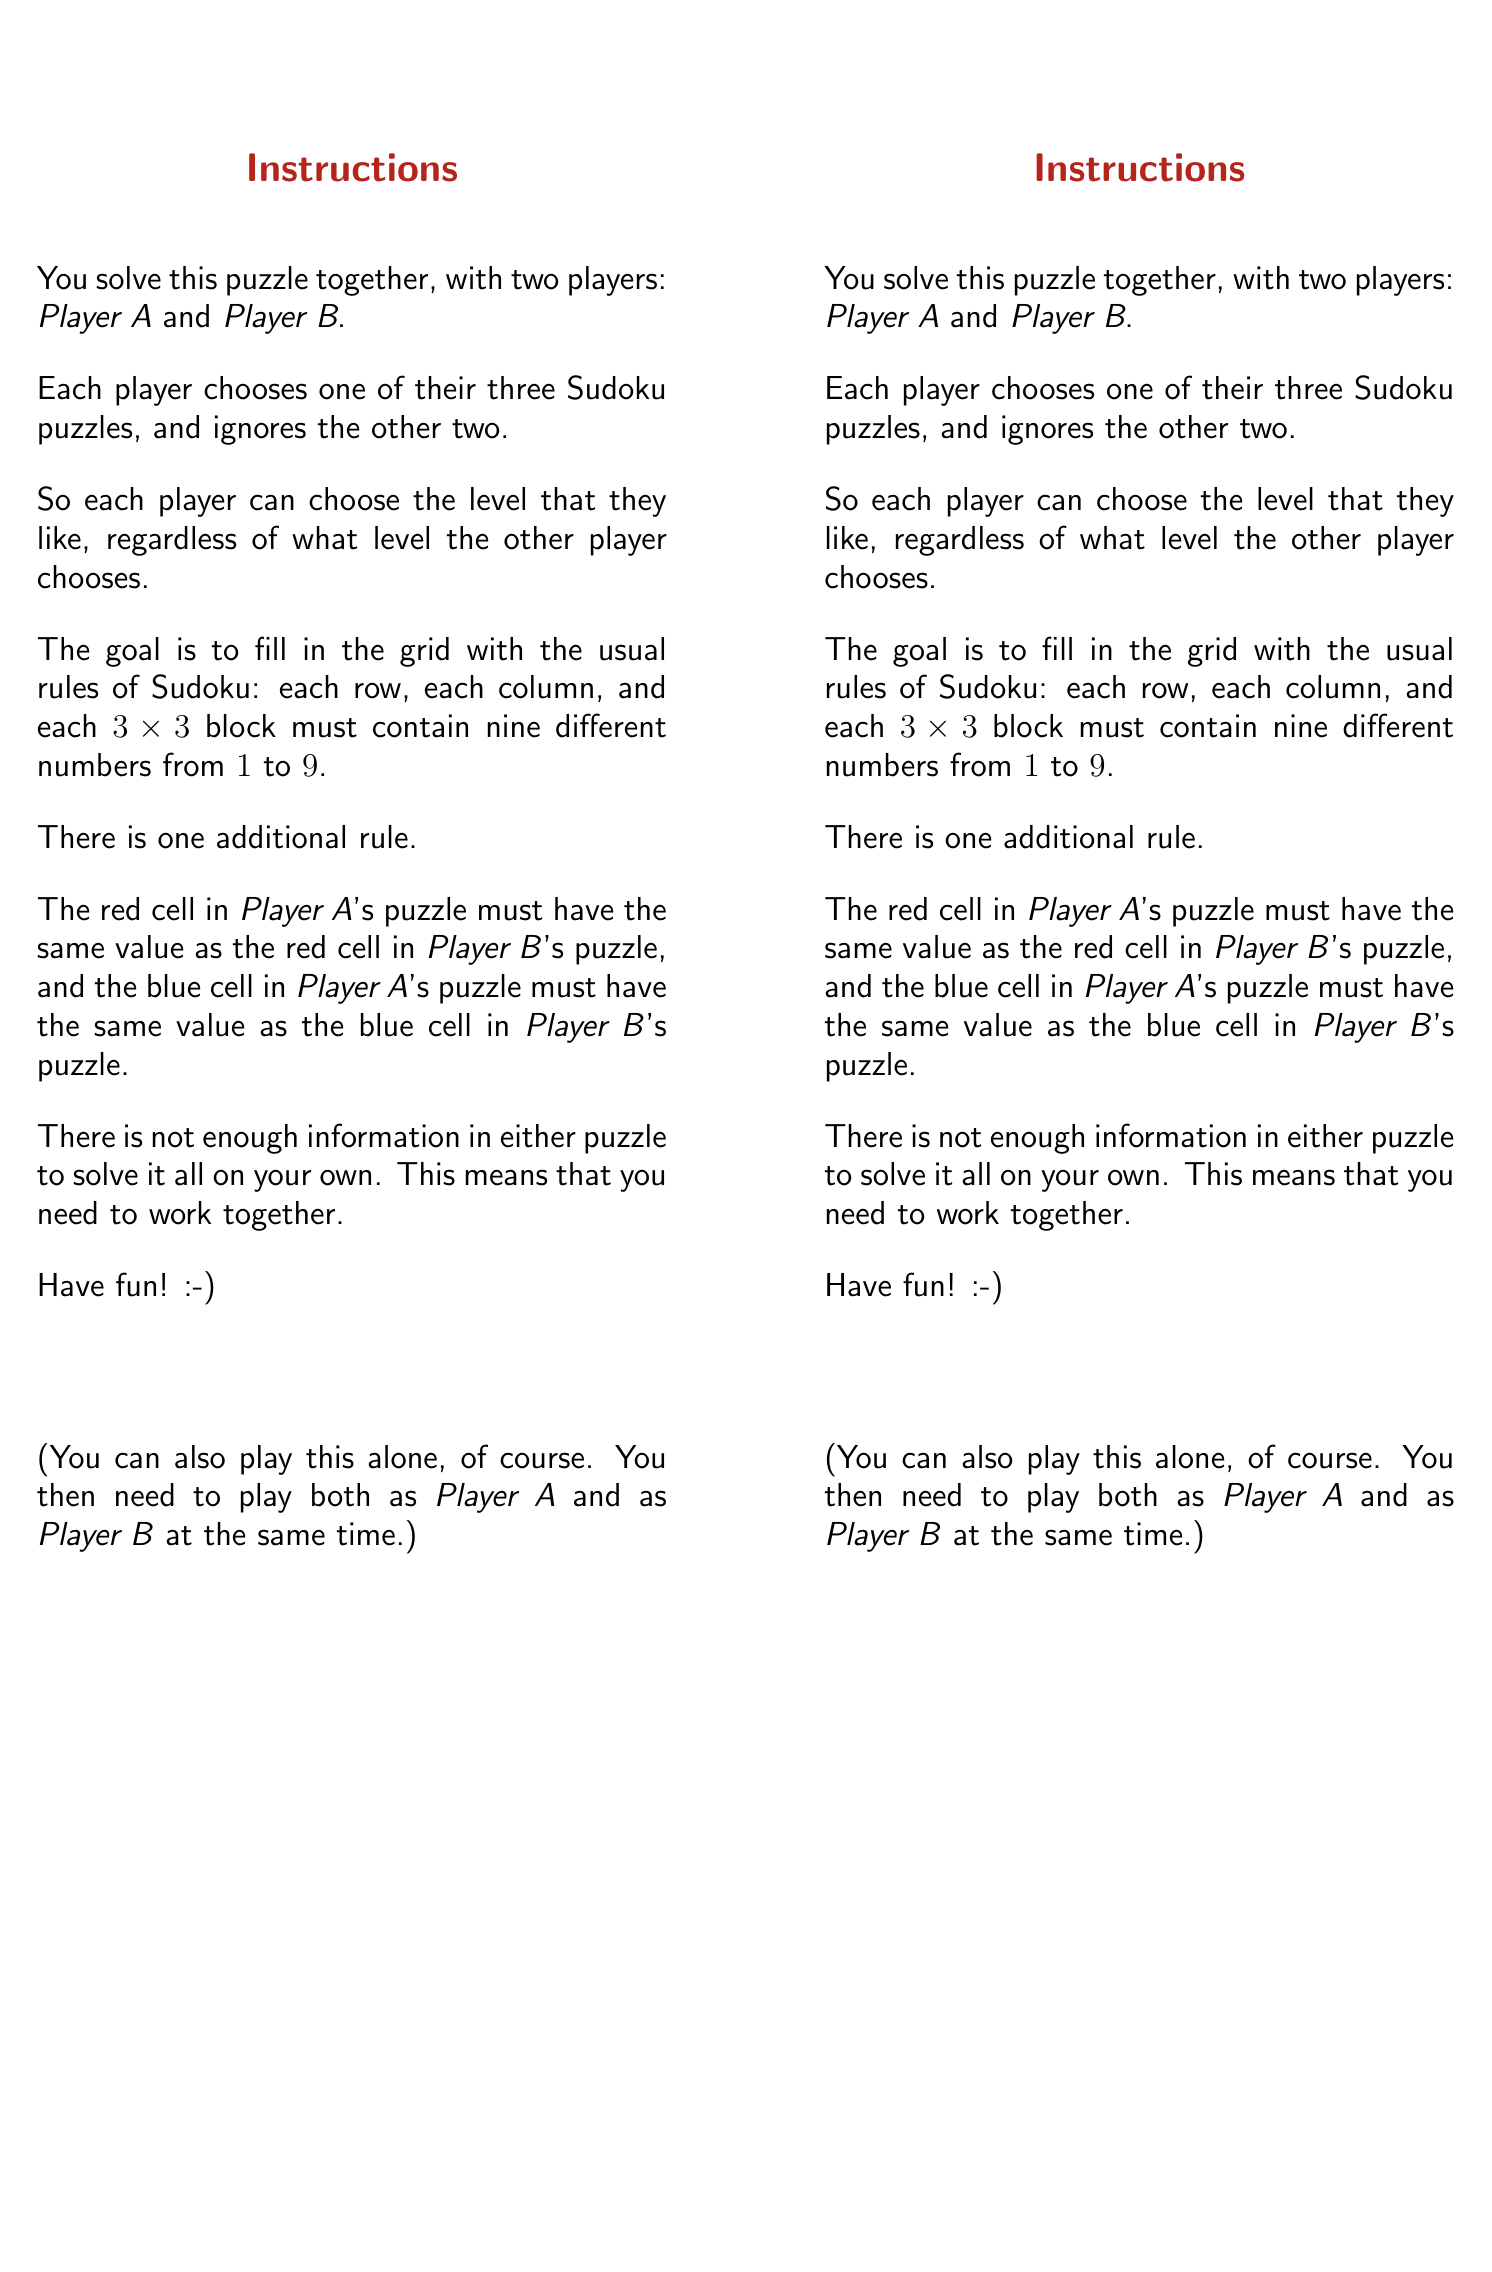
\begin{tikzpicture}
  %
  % PLAYER A
  \node[] at (-5,-1.25) {\parbox{5cm}{\centering \sffamily \Large \color{BrickRed} \textbf{Instructions}}};
  \node[] at (-5,-15) {\begin{minipage}[t][25.0cm][t]{8.0cm}\sffamily \large
  You solve this puzzle together, with two players: \textit{Player~A} and \textit{Player~B}.
  
  \bigskip
  
  Each player chooses one of their three Sudoku puzzles, and ignores the other two.
  
  \bigskip
  
  So each player can choose the level that they like,
  regardless of what level the other player chooses.
  
  \bigskip
  
  The goal is to fill in the grid with the usual rules of Sudoku:
  each row, each column, and each $3 \times 3$ block must contain
  nine different numbers from~$1$ to~$9$.
  
  \bigskip
  
  There is one additional rule.
  
  \bigskip
  
  The red cell in \textit{Player~A}'s puzzle must have the same value as the red
  cell in \textit{Player~B}'s puzzle,
  and the blue cell in \textit{Player~A}'s puzzle must have the same value as the blue
  cell in \textit{Player~B}'s puzzle.
  
  \bigskip
  
  There is not enough information in either puzzle to solve it all on your own.
  This means that you need to work together.
  
  \bigskip
  
  Have fun! :-)
  
  \bigskip\bigskip\bigskip\bigskip
  
  (You can also play this alone, of course. You then need to play both as
  \textit{Player~A} and as \textit{Player~B} at the same time.)
  
  \vfill
  \end{minipage}};
  % PLAYER B
  \node[] at (5,-1.25) {\parbox{5cm}{\centering \sffamily \Large \color{BrickRed} \textbf{Instructions}}};
  \node[] at (5,-15) {\begin{minipage}[t][25.0cm][t]{8.0cm}\sffamily \large
  You solve this puzzle together, with two players: \textit{Player~A} and \textit{Player~B}.
  
  \bigskip
  
  Each player chooses one of their three Sudoku puzzles, and ignores the other two.
  
  \bigskip
  
  So each player can choose the level that they like,
  regardless of what level the other player chooses.
  
  \bigskip
  
  The goal is to fill in the grid with the usual rules of Sudoku:
  each row, each column, and each $3 \times 3$ block must contain
  nine different numbers from~$1$ to~$9$.
  
  \bigskip
  
  There is one additional rule.
  
  \bigskip
  
  The red cell in \textit{Player~A}'s puzzle must have the same value as the red
  cell in \textit{Player~B}'s puzzle,
  and the blue cell in \textit{Player~A}'s puzzle must have the same value as the blue
  cell in \textit{Player~B}'s puzzle.
  
  \bigskip
  
  There is not enough information in either puzzle to solve it all on your own.
  This means that you need to work together.
  
  \bigskip
  
  Have fun! :-)
  
  \bigskip\bigskip\bigskip\bigskip
  
  (You can also play this alone, of course. You then need to play both as
  \textit{Player~A} and as \textit{Player~B} at the same time.)
  \vfill
  \end{minipage}};
  %
  \draw[] (0,0.5) edge[ultra thick, dashed,white] (0,-27);
  %
\end{tikzpicture}
\end{center}

\end{document}
